\documentclass[11pt, spanish]{article}
\usepackage[utf8]{inputenc}
\usepackage{listings} 
\usepackage{graphicx}
\usepackage{amsfonts}
\usepackage[dvipsnames]{xcolor}
\usepackage[T1]{fontenc}
\usepackage{bigfoot}
\usepackage{amsmath}
\usepackage[numbered,framed]{matlab-prettifier}
\usepackage{caption}
\usepackage[figurename=Figura, tablename=Tabla, font={small,tt}]{caption}
\usepackage{blkarray}
\usepackage{xcolor}
\usepackage{multicol}
\usepackage[]{algorithm2e}
\usepackage{float}

\makeatletter
    \setlength\@fptop{0\p@}
\makeatother

\date{}

\usepackage{geometry}
 \geometry{
 a4paper,
 left=30mm,
 right=30mm,
 top=30mm,
 }

\lstset{
	style              = Matlab-editor,
  	basicstyle         = \mlttfamily,
  	escapechar         = ",
  	mlshowsectionrules = true,
	framesep=4.5mm,
	framexleftmargin=2.5mm,
	fillcolor=\color{White},
	rulecolor=\color{Black},
	numberstyle=\normalfont\tiny\color{Black}
}

\captionsetup[lstlisting]{font={small,tt}}
\renewcommand{\lstlistingname}{Script}
\newcommand\RED{\color{red}}
\newcommand\BLUE{\color{blue}}
\newcommand{\BigO}[1]{\ensuremath{\operatorname{O}\bigl(#1\bigr)}}
\newcommand{\norm}[1]{\left\lVert#1\right\rVert}

\begin{document}

\renewcommand\lstlistlistingname{Lista de Scripts}

\author{Sebastián Valencia Calderón \\ 201111578}
\title{Laboratorio 5: Manejo de polinomios en \textsc{Matlab}.}
\maketitle

%====================================================================
\section{Introducción}

Los polinomios son estructuras algebraicas que relacionan números complejos a través de la suma de términos no lineales sobre la variable perteneciente al dominio de la función. La estructura de los polinomios es tan versátil que además de ser una función continua y diferenciable, el conjunto de los polinomios con las operaciones fundamentales sobre ellas, constituye un espacio vectorial. Por esta misma naturaleza, los polinomios pueden ser tratados como estructuras discretas, lo que resulta ideal y pertinente para un óptimo tratamiento de ellos usando un computador digital. Existe una gran variedad de algoritmos fundamentales que hacen parte de un conjunto de algoritmos útiles para el tratamiento de polinomios y otras estructuras en áreas como computación científica, comunicaciones, procesamiento de señales, estadística, etc.\\

Una notación conveniente para el tratamiento de polinomios es la siguiente:

$$P_n(x) = a_nx^n + a_{n-1}x^{n-1} + \dots + a_{1}x + a_{0} = \sum_{i = 0}^{n}a_{i}x^i$$

La última parte de la igualdad, sugiere la siguiente representación:

$$\begin{bmatrix}
    a_{0} & a_{1}  & \dots & a_{n - 1} & a_n 
\end{bmatrix} 
\begin{bmatrix}
    1 \\
    x \\
    \vdots \\
    x^{n-1} \\
    x^n    
\end{bmatrix} =  \sum_{i = 0}^{n}a_{i}x^i$$

El vector fila de la anterior relación, sugiere una representación vectorial de los coeficientes del polinomio, este vector contiene toda la información del polinomio, el grado y los coeficientes. Con esta representación vectorial, es fácil tratar y almacenar polinomios. De hecho, esta es la representación de polinomios en \textsc{Matlab}. Dado un polinomios, conviene realizar las operaciones básicas sobre el (suma, resta, producto, división, evaluación, derivación y hallar las raíces de un polinomio). El desarrollo de este laboratorio, pretende explorar la representación y manipulación de polinomios en \textsc{Matlab}. El desarrollo de estos ejercicios, pretende comprometerse con los siguientes objetivos:

\begin{enumerate}
\item Introducir de forma experimental algunos de los conceptos relacionados con el cálculo de raíces de un polinomio de grado $n$.
\item Identificar la representación de polinomios de cual hace uso \textsc{Matlab} y su relación con el álgebra matricial.
\item Reconocer algunas de las funciones incluidas en \textsc{Matlab} para trabajar con polinomios.
\end{enumerate}

%==================================================================
\section{Procedimiento}

Para cumplir los objetivos enumerados anteriormente, se desarrollan ejercicios propuestos sobre ciertos algoritmos, hallando las relaciones obtenidas a partir de ellos mediante el uso de suma, productor, división y diferenciación. Para cada uno de estos polinomios, se evalúa el mismo en un rango pertinente y se gráfica cada uno de ellos. Además, las raíces de los mismos se hallan y se grafican en el plano complejo.\\

 El desarrollo de cada uno de estos ejercicios, requiere comprender el funcionamiento y concepto de cada una de las funciones dispuestas en \textsc{Matlab} para el manejo de polinomios. El desarrollo del laboratorio, comienza con la comprensión de cada uno de estos métodos o funciones.

%==================================================================
\section{Resultados}

A continuación, se exponen los resultados, las metodologías propuestas para los análisis y las herramientas de ejecución para cada uno de los problemas propuestos.

\subsection{Manejo de polinomios en \textsc{Matlab}}
Se estudia la documentación sobre el uso y los conceptos involucrados en las funciones más relevantes para el manejo de polinomios en \textsc{Matlab}. La referencia principal para entender cada uno de estos procedimientos, es \cite{lopez2014matlab}, y \cite{yang2005applied}. Los ejemplos, fueron obtenidos en la documentación de \textsc{Matlab}.

\begin{itemize}

\item \texttt{roots(p)}: retorna a manera de vector, las raíces de un polinomio cuya representación está dada por el vector columna $p$. El vector de entrada, consiste en el vector en $\begin{bmatrix} a_{0} & a_{1}  & \dots & a_{n - 1} & a_n 
\end{bmatrix} \in \mathbb{R}^{n+1}$, el cual a su vez, representa un polinomio $P_n(x) = a_nx^n + a_{n-1}x^{n-1} + \dots + a_{1}x + a_{0}$. La función \texttt{roots(p)}, resuelve la ecuación $a_nx^n + a_{n-1}x^{n-1} + \dots + a_{1}x + a_{0} = 0$, donde la variable $x$, no posee exponentes negativos. Un ejemplo de uso es: \\

\lstinputlisting[caption = {}]{data/scripts/usage/usageroots.m}\

Ahora la variable $r$, contienen los números complejos que satisfacen la ecuación $x^4 - 1 = 0$. Para calcular las raices, del polinomio, \textsc{Matlab} calcula los valores propios de una matriz cuya diagonal contiene los coeficientes del vector $p$.

\item \texttt{conv(p, q)}: retorna la convolución (en el contexto de procesamiento de imagenes, la convolución representa el área en la que dos vectores $u$ y $v$ se traslapan. Algebraicamente, es una operación equivalente a la multiplicación de polinomios) de dos vectores. El parámetro opcional \texttt{shape}, especifica si el vector resultante debe tener el tamño de alguno de sus dos parámetros. Si éste último es \texttt{same}, retorna la misma parte que $p$, si es \texttt{valid}, retorna la parte de la convolución sin ceros en los extremos. Si se quiere multiplicar los polinomios $x^2+1$ y $2x + 7$ en \textsc{Matlab}, se debe ejecutar las siguientes instrucciones.\\

\lstinputlisting[caption = {}]{data/scripts/usage/usageconv.m}\

Ahora la variable $w$, contiene una representación del polinomio $2\, x^3 + 7\, x^2 + 2\, x + 7$.

\item \texttt{deconv(p, q)}: aplica el proceso inverso a la deconvolución entre los vectores $p$ y $q$, haciendo uso de división larga. El vector cociente, es devuelto en el primer valor de retorno, y el residuo en el segundo, de tal manera, $p = \texttt{conv(q, quatient)} + \texttt{remainder}$. El siguiente script, se ejecuta para demostrar el funcionamiento de \texttt{deconv(p, q)}, y para verificar este hecho:\\

\lstinputlisting[caption = {}]{data/scripts/usage/usagedeconv.m}\

La variable $c$, toma un valor para representar el polinomio $10\, x^5 + 40\, x^4 + 100\, x^3 + 160\, x^2 + 170\, x + 120$, la variable $q$, representa el polinomio $10\, x^2 + 20\, x + 30$, y $r  =  0$. Es fácil verificar que $c = \texttt{conv(u, q)} + \texttt{r}$.

\item \texttt{polyder(p)}: retorna la derivada del polinomio $p$, determinada por el orden y los coeficientes del mismo. Un segundo parámetro asignado a únicamente una variable ($\texttt{k} = \texttt{polyder(a, b)}$), representa la derivada del producto de dos polinomios, mientras que la función aplicada a dos argumentos y asignada a un vector de dos elementos ($\texttt{[q, d]} = \texttt{polyder(a, b)}$), retorna la derivada del cociente entre dos polinomios. Dado que el primer uso puede ser usado para calcular los otros dos, se incluye un script ejemplificando este primer caso.\\

\lstinputlisting[caption = {}]{data/scripts/usage/usagepolyder.m}\

En este caso, $p$, representa al polinomio $3\, x^5 - 2\, x^3 + x + 5$, del cual su derivada es $15\, x^4 - 6\, x^2 + 1$, representada en el vector $q$.

\item \texttt{polyval(p, x)}: retorna el valor de evaluación del polinomio $p$, de grado $n$, en el valor $x$, es decir, reemplaza la variable del polinomio por el valor de $x$ y calcula la suma de términos. A continuación, se ejemplifica su uso:\\

\lstinputlisting[caption = {}]{data/scripts/usage/usagepolyval.m}\

Después de la ejecución de las instrucciones anteriores, $p$, representa el polinomio $3\, x^2 + 2\, x + 1$, cuyo valor en $x = 2$, es $17$, y es el valor de la variable $x$.

\end{itemize}

\subsection{Aplicación de conceptos}

Sean:

$$f(x) = x^2+2x+3 \qquad g(x) = 9x^4+4x^3+3x^2+2x+1$$

\begin{enumerate}
\item La generación de polinomios, se logra a través de:\\

\lstinputlisting[caption = {}]{data/scripts/genpol.m}

\item Dados los vectores fila usados en el literal anterior para la generación y representación de los polinomios en \textsc{Matlab}, cada uno de estos representan los siguientes polinomios obtenidos con el siguiente script:\\

\lstinputlisting[caption = {}]{data/scripts/sympol.m}

El anterior script, da como resultado: \texttt{symf} = $x^2 + 2x + 3$, y \texttt{symg} = $9x^4 + 4x^3 + 3x^2 + 2x + 1$

\newpage
\item Los polinomios $f(x)$ y $g(x)$, pueden ser usados para obtener los siguientes polinomios:

\begin{itemize}
\item $h(x) = f(x) \times g(x)$
\item $k(x) = f(x)\ /\ g(x)$
\item $v(x) = \partial g(x)\ /\ \partial x$
\end{itemize}

En \textsc{Matlab}, estas operaciones se materializan en el siguiente script.\\

\lstinputlisting[caption = {}]{data/scripts/genpoldec.m}

La representación simbólica de los polinomios obtenidos es:\\

\texttt{h(x)} = $9\, x^6 + 22\, x^5 + 38\, x^4 + 20\, x^3 + 14\, x^2 + 8\, x + 3$.\\

\texttt{kq(x)} = $0$, \texttt{kr(x)} = $x^2 + 2\, x + 3$.\\

\texttt{v(x)} = $36\, x^3 + 12\, x^2 + 6\, x + 2$.

\item Por medio de la función \texttt{root(p)}, se hallan las raíces de cada uno de los polinomios dados o encontrados a partir de ellos:

\begin{itemize}
\item \textbf{Raíces de $f(x)$:} $$\texttt{roots(f)} = [-1.0000 \pm 1.4142i]$$

\item \textbf{Raíces de $g(x)$:} $$\texttt{roots(g)} = [0.2021 \pm 0.5956i   \qquad -0.4244 \pm 0.3174i]$$

\item \textbf{Raíces de $h(x)$:} $$\texttt{roots(h)} = [-1.0000 \pm 1.4142i    \qquad 0.2021 \pm 0.5956i   \qquad -0.4244 -\pm 0.3174i]$$

\item \textbf{Raíces de $kr(x)$:} $$\texttt{roots(kr)} = [-1.0000 \pm 1.4142i]$$

\item \textbf{Raíces de $v(x)$:} $$\texttt{roots(v)} = [-0.0000 \pm 0.4082i  \qquad -0.3333]$$

\end{itemize}

\newpage

\item A continuación, se gráfica cada uno de los polinomios, y sus raíces en el plano complejo. Para esto, se hace uso de la siguiente función definida en \textsc{Matlab} para este propósito (es necesario incluir la función, ya que es quien usa directamente las funciones \texttt{roots}, y \texttt{polyval}). Para el posicionamiento y despliegue de cada una de las graficas, se uso la referencia \cite{jaluria2011computer}, y la referencia \cite{siauw2014introduction}.\\

\lstinputlisting[caption = {}]{data/scripts/plotpolroots.m}

\newpage

\begin{itemize}
\item \textbf{Gráfica y raíces de $f(x)$} A través de la invocación: \texttt{plotpolroots(f, 'f', 'y', -100, 100)}

\begin{figure}[H]
\centering
	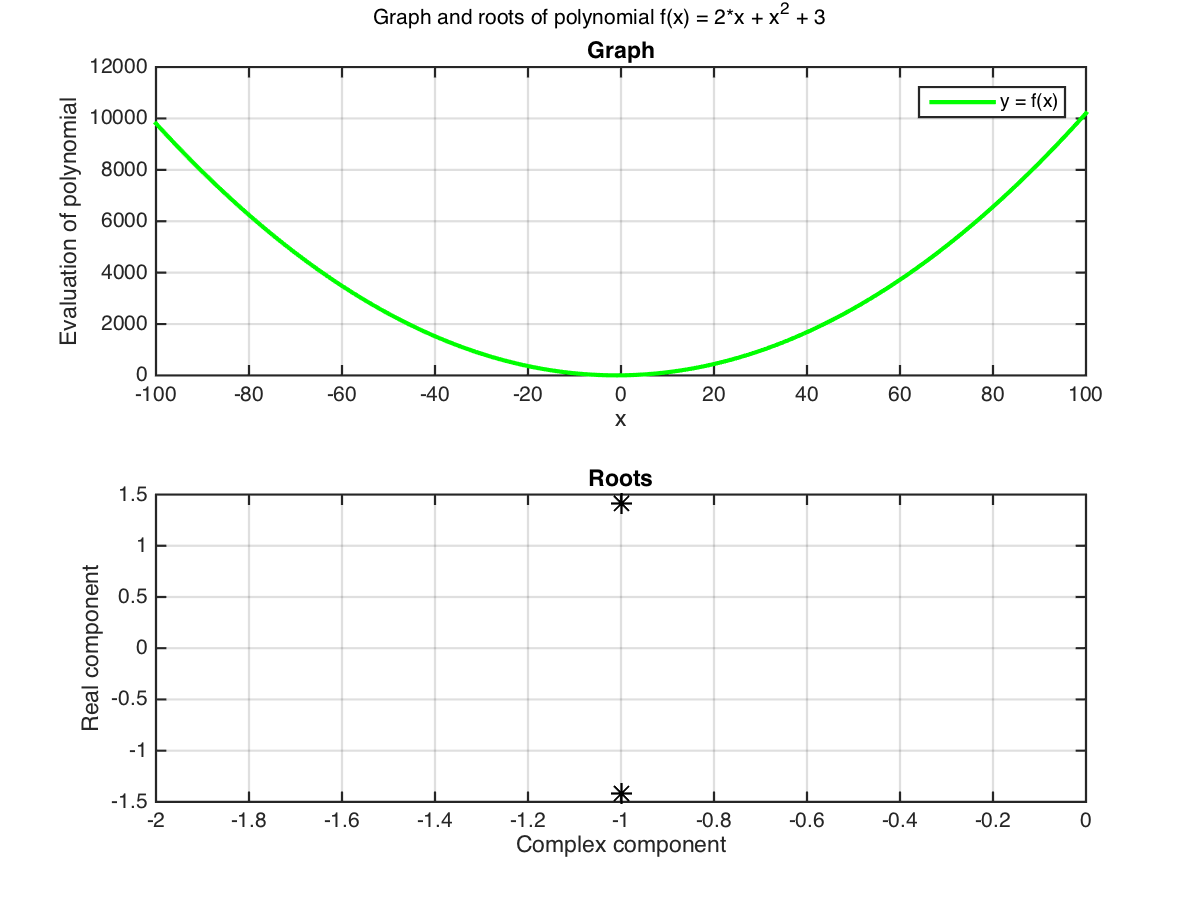
\includegraphics[scale=0.6]{data/img/fplot}
	\caption{}
\end{figure}

\item \textbf{Gráfica y raíces de $g(x)$} A través de la invocación: \texttt{plotpolroots(g, 'g', 'm', -1000, 1000)}

\begin{figure}[H]
\centering
	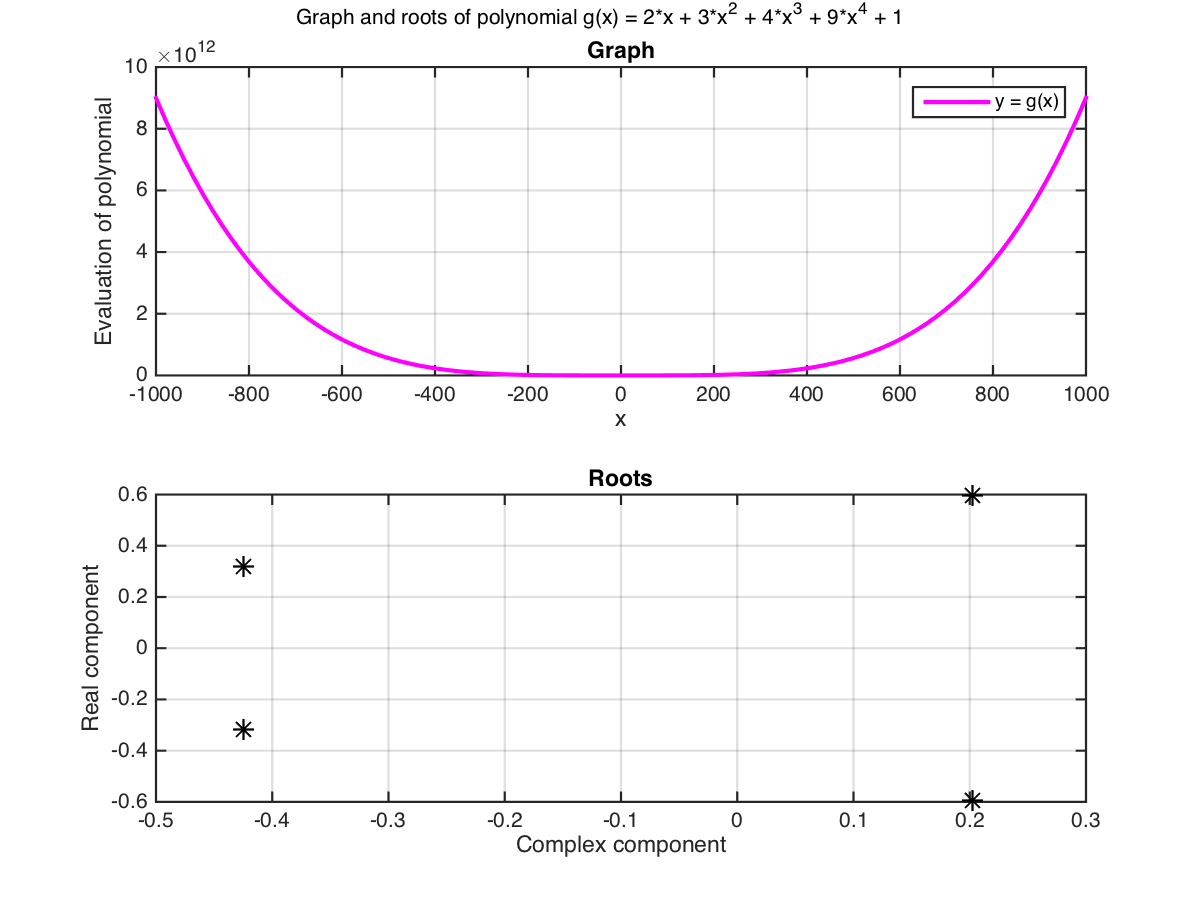
\includegraphics[scale=0.6]{data/img/gplot}
	\caption{}
\end{figure}

\newpage

\item \textbf{Gráfica y raíces de $h(x)$} A través de la invocación: \texttt{plotpolroots(h, 'h', 'c', -1000, 1000)}

\begin{figure}[H]
\centering
	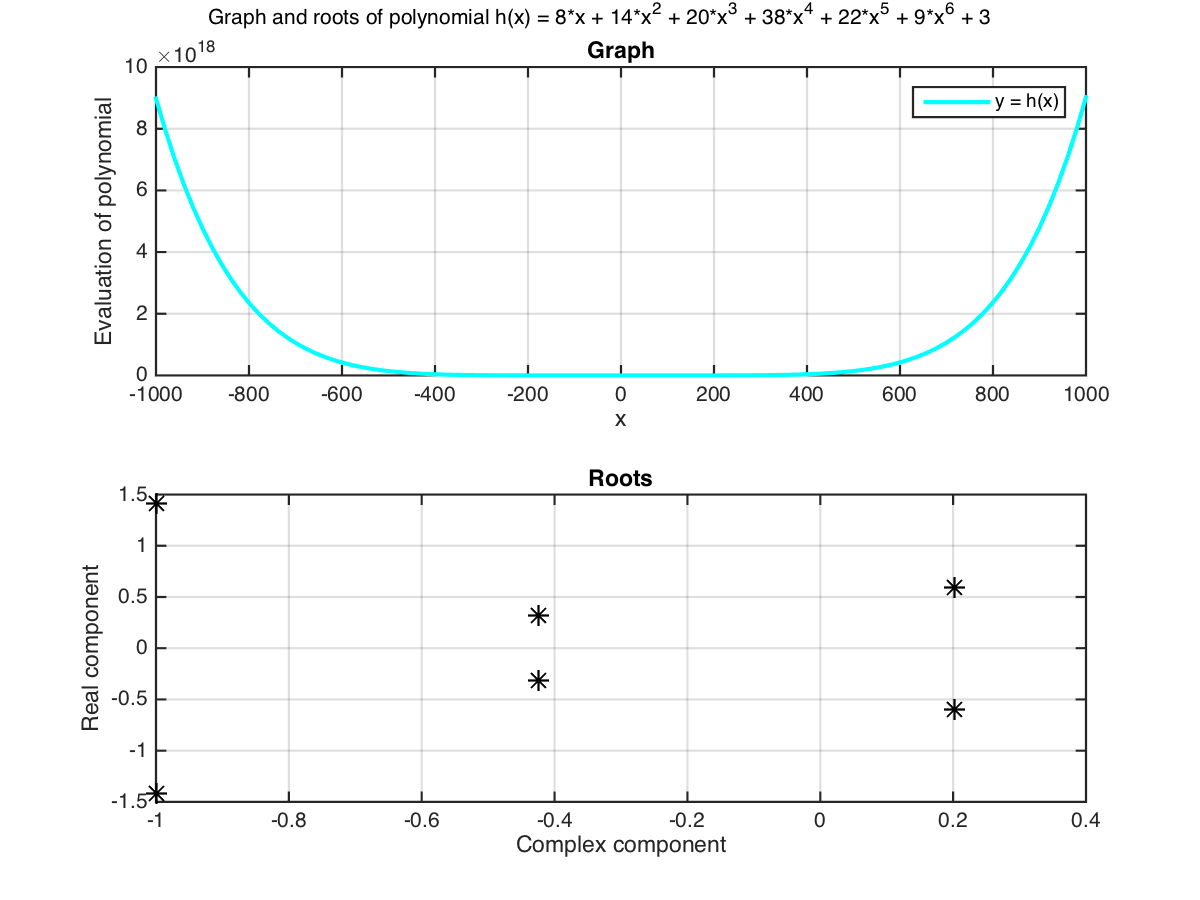
\includegraphics[scale=0.6]{data/img/hplot}
	\caption{}
\end{figure}

\item \textbf{Gráfica y raíces de $kr(x)$} A través de la invocación: \texttt{plotpolroots(kr, 'kr', 'r', -100, 100)}

\begin{figure}[H]
\centering
	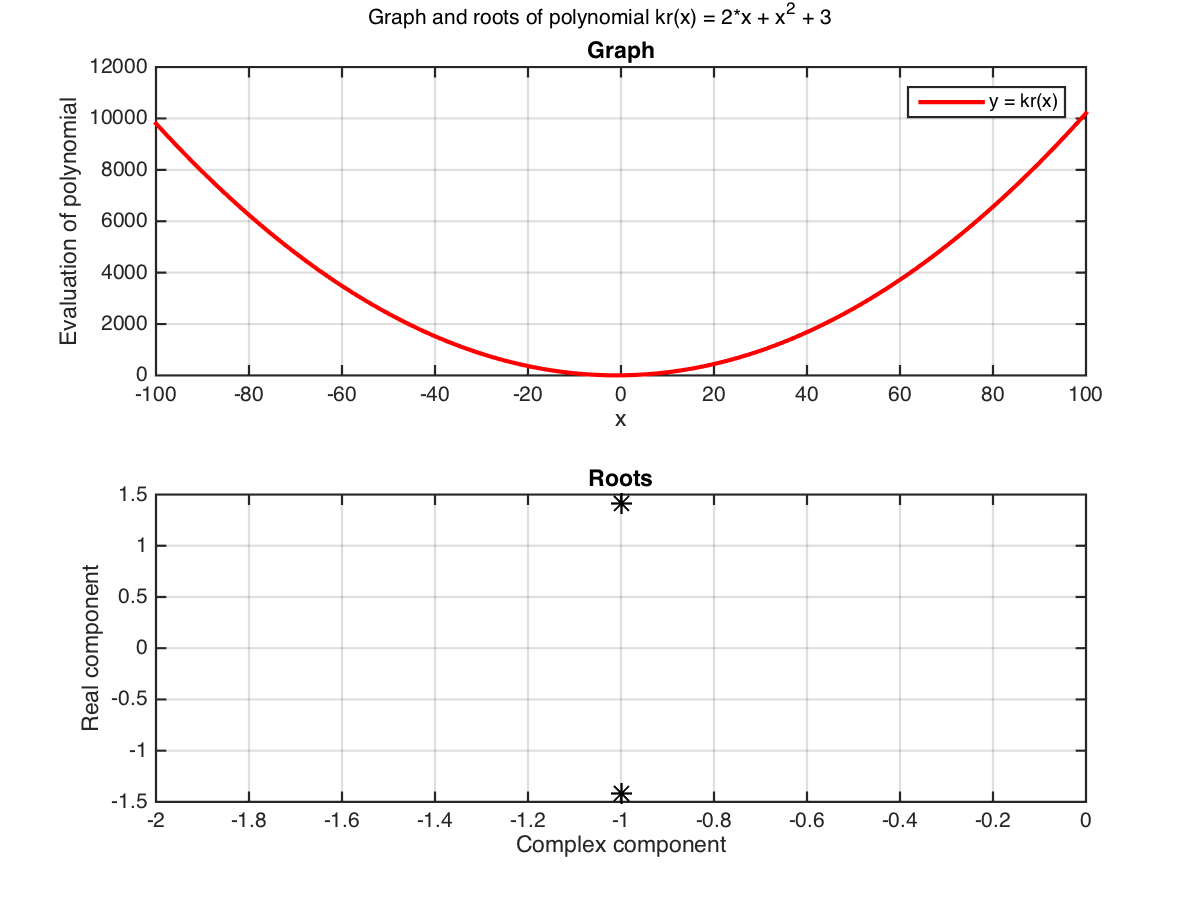
\includegraphics[scale=0.6]{data/img/krplot}
	\caption{}
\end{figure}

\newpage

\item \textbf{Gráfica y raíces de $v(x)$} A través de la invocación: \texttt{plotpolroots(v, 'v', 'b', -100, 100)}

\begin{figure}[H]
\centering
	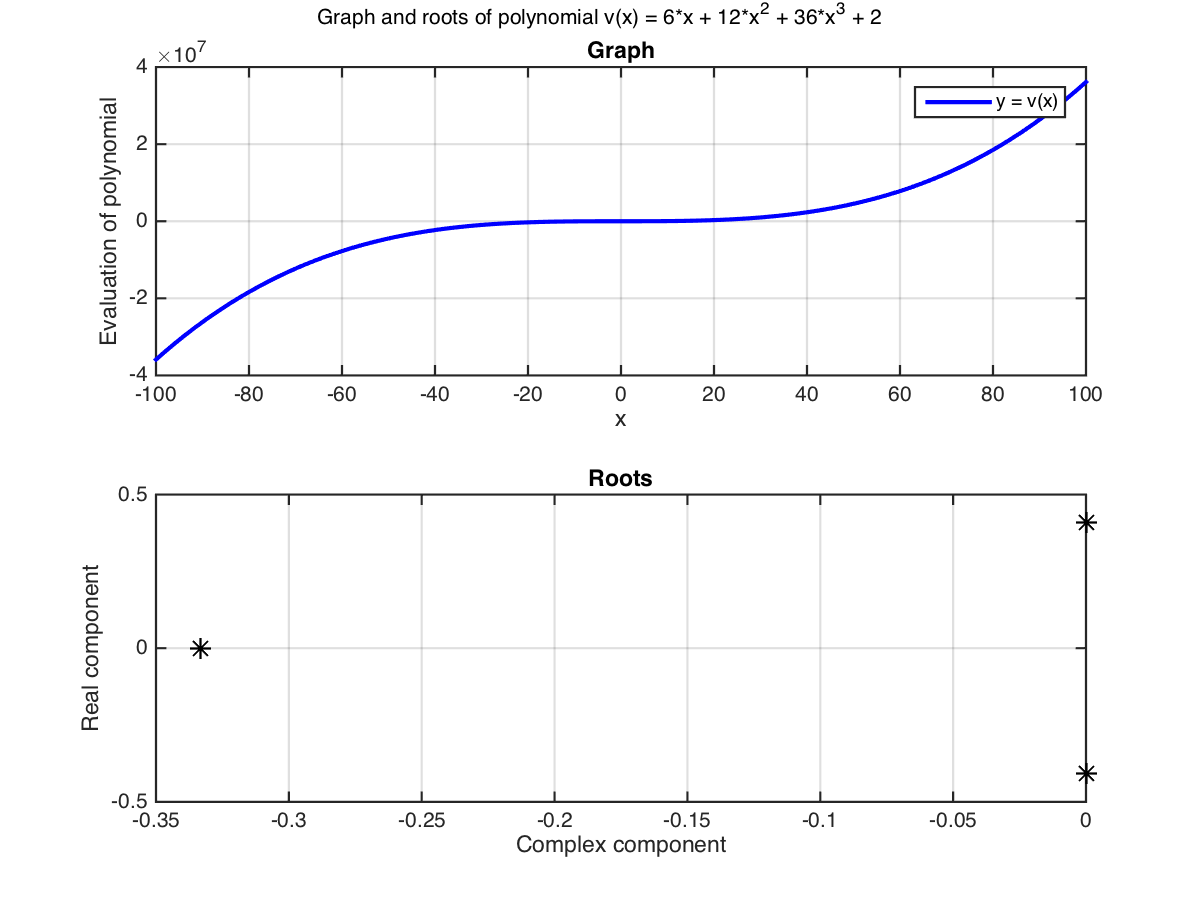
\includegraphics[scale=0.6]{data/img/vplot}
	\caption{}
\end{figure}

\end{itemize}

\item Por último, se hace uso de la función \texttt{factor}, para clasificar las raíces  de cada uno de los polinomios. Para cada uno de los polinomios, se ejecuta la instrucción \texttt{factor(poly2sym(pol), x, 'FactorMode', 'complex')}, donde \texttt{pol}, es la variable que apunta a la representación del polinomio de cada caso:

\begin{itemize}
\item \textbf{Raíces de $f(x)$} \\

\texttt{[ x + 1.0 - 1.414i, x + 1.0 + 1.414i]}

\item \textbf{Raíces de $g(x)$} \\

\texttt{[ 9.0, x - 0.202 + 0.595i, x + 0.424 + 0.317, x - 0.202 - 0.595i, x + 0.424 - 0.317i]}

\item \textbf{Raíces de $h(x)$} \\

\texttt{[ 9.0, x + 1.0 - 1.414i, x - 0.202 + 0.595i, x + 0.424 + 0.317i, x + 1.0 + 1.414i, x - 0.202 - 0.595i, x + 0.424 - 0.317i]}

\item \textbf{Raíces de $kr(x)$} \\

\texttt{[ x + 1.0 - 1.414i, x + 1.0 + 1.414i]}

\item \textbf{Raíces de $v(x)$} \\

\texttt{[ 36.0, x + 0.333, x - 0.408i, x + 0.408i]}

\end{itemize}

\end{enumerate}
%==================================================================
\newpage
\section{Conclusiones}

El desarrollo de los ejercicios propuestos para el laboratorio, sirvieron para conceptualizar los algoritmos fundamentales para el tratamiento de una estructura algebraica fundamental tal y como son los polinomios. Entender el manejo de polinomios en \textsc{Matlab}, es fundamental, pues muchos problemas relacionados con la solución numérica de ecuaciones diferenciales ordinarias y parciales, pueden reducirse a problemas relacionados con polinomios. Además, resulta práctico obtener las raíces de un polinomio de grado mayor a dos, pues con cierta tolerancia numérica, se obtienen los ceros de un polinomio. Esto resulta interesante, si se considera que para polinomios de grado mayor o igual a cinco, es una tara imposible hallar expresiones algebraicas para determinar las raíces del polinomio (Galois y Abel). \\

Es interesante ver que \textsc{Matlab}, el cual obtiene su nombre gracias a la expresión \textit{Matrix laboratory}, reduce los problemas de polinomios a problemas matriciales, pues como se documento, hallar las raíces de un polinomio, es tratado en la plataforma como encontrar los valores propios de una matriz cuyos elementos de la diagonal, son los elementos del vector que representa el polinomio. Aparte de esto, la representación vectorial de polinomios en \textsc{Matlab}, sugiere también este hecho. De manera puntual, cabe resaltar a manera de conclusión lo siguiente:

\begin{itemize}

\item Los ejercicios cuyo objetivo fue el de familiarizar al usuario con la administración de polinomios en \textsc{Matlab}, sirvieron para afianzar los conceptos fundamentales sobre las operaciones principales sobre polinomios. Resulto inquietante la conveniente representación interna de los polinomios en \textsc{Matlab}, lo cual ayuda con la eficiencia y escritura de las operaciones antes mencionadas.
   
\end{itemize}


%==================================================================

\section{Bibliografía}

\begingroup
\renewcommand{\section}[2]{}%
\begin{thebibliography}{}

% Matlab Bibliography

\bibitem{jaluria2011computer} Jaluria, Y. {\em Computer Methods for Engineering with MATLAB Applications, Second Edition.} 2011. Series in Computational and Physical Processes in Mechanics and Thermal Sciences - Taylor \& Francis. Pags. 60 - 63.

\bibitem{yang2005applied} Yang, W.Y. and Cao, W. and Chung, T.S. and Morris, J. {\em Applied Numerical Methods Using MATLAB.} 2005. Wiley. Pags. 50 - 57.

\bibitem{lopez2014matlab} Lopez, C. {\em MATLAB Symbolic Algebra and Calculus Tools.} 2014. MATLAB Solutions Series - Apress. Pags. 73 - 75.

\bibitem{siauw2014introduction} Siauw, T. and Bayen, A. {\em An Introduction to MATLAB Programming and Numerical Methods for Engineers} 2014. Elsevier Science. Pags. 198 - 200.

\end{thebibliography}
\endgroup

\bibliography{sample}

\end{document}
